\documentclass[twoside]{book}

% Packages required by doxygen
\usepackage{fixltx2e}
\usepackage{calc}
\usepackage{doxygen}
\usepackage[export]{adjustbox} % also loads graphicx
\usepackage{graphicx}
\usepackage[utf8]{inputenc}
\usepackage{makeidx}
\usepackage{multicol}
\usepackage{multirow}
\PassOptionsToPackage{warn}{textcomp}
\usepackage{textcomp}
\usepackage[nointegrals]{wasysym}
\usepackage[table]{xcolor}

% Font selection
\usepackage[T1]{fontenc}
\usepackage[scaled=.90]{helvet}
\usepackage{courier}
\usepackage{amssymb}
\usepackage{sectsty}
\renewcommand{\familydefault}{\sfdefault}
\allsectionsfont{%
  \fontseries{bc}\selectfont%
  \color{darkgray}%
}
\renewcommand{\DoxyLabelFont}{%
  \fontseries{bc}\selectfont%
  \color{darkgray}%
}
\newcommand{\+}{\discretionary{\mbox{\scriptsize$\hookleftarrow$}}{}{}}

% Page & text layout
\usepackage{geometry}
\geometry{%
  a4paper,%
  top=2.5cm,%
  bottom=2.5cm,%
  left=2.5cm,%
  right=2.5cm%
}
\tolerance=750
\hfuzz=15pt
\hbadness=750
\setlength{\emergencystretch}{15pt}
\setlength{\parindent}{0cm}
\setlength{\parskip}{3ex plus 2ex minus 2ex}
\makeatletter
\renewcommand{\paragraph}{%
  \@startsection{paragraph}{4}{0ex}{-1.0ex}{1.0ex}{%
    \normalfont\normalsize\bfseries\SS@parafont%
  }%
}
\renewcommand{\subparagraph}{%
  \@startsection{subparagraph}{5}{0ex}{-1.0ex}{1.0ex}{%
    \normalfont\normalsize\bfseries\SS@subparafont%
  }%
}
\makeatother

% Headers & footers
\usepackage{fancyhdr}
\pagestyle{fancyplain}
\fancyhead[LE]{\fancyplain{}{\bfseries\thepage}}
\fancyhead[CE]{\fancyplain{}{}}
\fancyhead[RE]{\fancyplain{}{\bfseries\leftmark}}
\fancyhead[LO]{\fancyplain{}{\bfseries\rightmark}}
\fancyhead[CO]{\fancyplain{}{}}
\fancyhead[RO]{\fancyplain{}{\bfseries\thepage}}
\fancyfoot[LE]{\fancyplain{}{}}
\fancyfoot[CE]{\fancyplain{}{}}
\fancyfoot[RE]{\fancyplain{}{\bfseries\scriptsize Generated by Doxygen }}
\fancyfoot[LO]{\fancyplain{}{\bfseries\scriptsize Generated by Doxygen }}
\fancyfoot[CO]{\fancyplain{}{}}
\fancyfoot[RO]{\fancyplain{}{}}
\renewcommand{\footrulewidth}{0.4pt}
\renewcommand{\chaptermark}[1]{%
  \markboth{#1}{}%
}
\renewcommand{\sectionmark}[1]{%
  \markright{\thesection\ #1}%
}

% Indices & bibliography
\usepackage{natbib}
\usepackage[titles]{tocloft}
\setcounter{tocdepth}{3}
\setcounter{secnumdepth}{5}
\makeindex

% Hyperlinks (required, but should be loaded last)
\usepackage{ifpdf}
\ifpdf
  \usepackage[pdftex,pagebackref=true]{hyperref}
\else
  \usepackage[ps2pdf,pagebackref=true]{hyperref}
\fi
\hypersetup{%
  colorlinks=true,%
  linkcolor=blue,%
  citecolor=blue,%
  unicode%
}

% Custom commands
\newcommand{\clearemptydoublepage}{%
  \newpage{\pagestyle{empty}\cleardoublepage}%
}

\usepackage{caption}
\captionsetup{labelsep=space,justification=centering,font={bf},singlelinecheck=off,skip=4pt,position=top}

%===== C O N T E N T S =====

\begin{document}

% Titlepage & ToC
\hypersetup{pageanchor=false,
             bookmarksnumbered=true,
             pdfencoding=unicode
            }
\pagenumbering{alph}
\begin{titlepage}
\vspace*{7cm}
\begin{center}%
{\Large My Project }\\
\vspace*{1cm}
{\large Generated by Doxygen 1.8.13}\\
\end{center}
\end{titlepage}
\clearemptydoublepage
\pagenumbering{roman}
\tableofcontents
\clearemptydoublepage
\pagenumbering{arabic}
\hypersetup{pageanchor=true}

%--- Begin generated contents ---
\chapter{Class Index}
\section{Class List}
Here are the classes, structs, unions and interfaces with brief descriptions\+:\begin{DoxyCompactList}
\item\contentsline{section}{\hyperlink{structshmseg}{shmseg} \\*This is the message structure containing the id of the message writer and the message }{\pageref{structshmseg}}{}
\end{DoxyCompactList}

\chapter{File Index}
\section{File List}
Here is a list of all files with brief descriptions\+:\begin{DoxyCompactList}
\item\contentsline{section}{src/\hyperlink{shm__client2_8c}{shm\+\_\+client2.\+c} }{\pageref{shm__client2_8c}}{}
\item\contentsline{section}{src/\hyperlink{shm__server2_8c}{shm\+\_\+server2.\+c} }{\pageref{shm__server2_8c}}{}
\end{DoxyCompactList}

\chapter{Class Documentation}
\hypertarget{structshmseg}{}\section{shmseg Struct Reference}
\label{structshmseg}\index{shmseg@{shmseg}}


this is the message structure containing the id of the message writer and the message  


\subsection*{Public Attributes}
\begin{DoxyCompactItemize}
\item 
int \hyperlink{structshmseg_a1be1260af3aed063a18e121ab8f0e3a7}{id}
\item 
char \hyperlink{structshmseg_a1d156466dfeba6cf58be88a970dd88a4}{message} \mbox{[}256\mbox{]}
\end{DoxyCompactItemize}


\subsection{Detailed Description}
this is the message structure containing the id of the message writer and the message 

\subsection{Member Data Documentation}
\mbox{\Hypertarget{structshmseg_a1be1260af3aed063a18e121ab8f0e3a7}\label{structshmseg_a1be1260af3aed063a18e121ab8f0e3a7}} 
\index{shmseg@{shmseg}!id@{id}}
\index{id@{id}!shmseg@{shmseg}}
\subsubsection{\texorpdfstring{id}{id}}
{\footnotesize\ttfamily int shmseg\+::id}

\mbox{\Hypertarget{structshmseg_a1d156466dfeba6cf58be88a970dd88a4}\label{structshmseg_a1d156466dfeba6cf58be88a970dd88a4}} 
\index{shmseg@{shmseg}!message@{message}}
\index{message@{message}!shmseg@{shmseg}}
\subsubsection{\texorpdfstring{message}{message}}
{\footnotesize\ttfamily char shmseg\+::message}



The documentation for this struct was generated from the following files\+:\begin{DoxyCompactItemize}
\item 
src/\hyperlink{shm__client2_8c}{shm\+\_\+client2.\+c}\item 
src/\hyperlink{shm__server2_8c}{shm\+\_\+server2.\+c}\end{DoxyCompactItemize}

\chapter{File Documentation}
\hypertarget{shm__client2_8c}{}\section{src/shm\+\_\+client2.c File Reference}
\label{shm__client2_8c}\index{src/shm\+\_\+client2.\+c@{src/shm\+\_\+client2.\+c}}
{\ttfamily \#include $<$stdlib.\+h$>$}\newline
{\ttfamily \#include $<$sys/ipc.\+h$>$}\newline
{\ttfamily \#include $<$sys/shm.\+h$>$}\newline
{\ttfamily \#include $<$stdio.\+h$>$}\newline
{\ttfamily \#include $<$unistd.\+h$>$}\newline
{\ttfamily \#include $<$pthread.\+h$>$}\newline
{\ttfamily \#include $<$string.\+h$>$}\newline
{\ttfamily \#include $<$semaphore.\+h$>$}\newline
{\ttfamily \#include $<$fcntl.\+h$>$}\newline
Include dependency graph for shm\+\_\+client2.\+c\+:\nopagebreak
\begin{figure}[H]
\begin{center}
\leavevmode
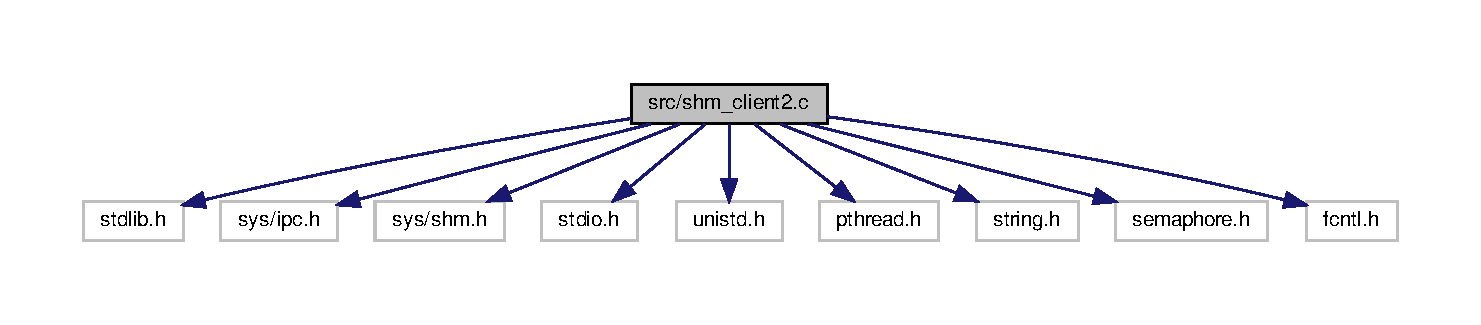
\includegraphics[width=350pt]{shm__client2_8c__incl}
\end{center}
\end{figure}
\subsection*{Classes}
\begin{DoxyCompactItemize}
\item 
struct \hyperlink{structshmseg}{shmseg}
\begin{DoxyCompactList}\small\item\em this is the message structure containing the id of the message writer and the message \end{DoxyCompactList}\end{DoxyCompactItemize}
\subsection*{Functions}
\begin{DoxyCompactItemize}
\item 
void $\ast$ \hyperlink{shm__client2_8c_af825808a184ae13bc67c961b0ed1a377}{func\+\_\+write} (void $\ast$args)
\item 
void $\ast$ \hyperlink{shm__client2_8c_ace3f9ecb971163860b43eb90bcd75ff2}{func\+\_\+read} (void $\ast$args)
\item 
int \hyperlink{shm__client2_8c_ae66f6b31b5ad750f1fe042a706a4e3d4}{main} ()
\end{DoxyCompactItemize}
\subsection*{Variables}
\begin{DoxyCompactItemize}
\item 
pthread\+\_\+mutex\+\_\+t \hyperlink{shm__client2_8c_a0abaf4b5d42c4e5d19190035fade3599}{lock}
\begin{DoxyCompactList}\small\item\em this the mutex to maintain lock between the threads \end{DoxyCompactList}\end{DoxyCompactItemize}
\textbf{ }\par
\begin{DoxyCompactItemize}
\item 
sem\+\_\+t $\ast$ \hyperlink{shm__client2_8c_a31dc0ff5363c41ad195f7e27d2d10ca9}{read\+\_\+block}
\begin{DoxyCompactList}\small\item\em these are the read and write semaphore pointers to maintain exclusivity between the server and client processes \end{DoxyCompactList}\item 
sem\+\_\+t $\ast$ \hyperlink{shm__client2_8c_a1ba04b4da8bf3354235de7186f980e7c}{write\+\_\+block}
\begin{DoxyCompactList}\small\item\em these are the read and write semaphore pointers to maintain exclusivity between the server and client processes \end{DoxyCompactList}\end{DoxyCompactItemize}



\subsection{Function Documentation}
\mbox{\Hypertarget{shm__client2_8c_ace3f9ecb971163860b43eb90bcd75ff2}\label{shm__client2_8c_ace3f9ecb971163860b43eb90bcd75ff2}} 
\index{shm\+\_\+client2.\+c@{shm\+\_\+client2.\+c}!func\+\_\+read@{func\+\_\+read}}
\index{func\+\_\+read@{func\+\_\+read}!shm\+\_\+client2.\+c@{shm\+\_\+client2.\+c}}
\subsubsection{\texorpdfstring{func\+\_\+read()}{func\_read()}}
{\footnotesize\ttfamily void$\ast$ func\+\_\+read (\begin{DoxyParamCaption}\item[{void $\ast$}]{args }\end{DoxyParamCaption})}

this function is the read function used by the read thread 
\begin{DoxyParams}{Parameters}
{\em args} & it contains the address of the shared memory shared between the server and the client \\
\hline
\end{DoxyParams}
\mbox{\Hypertarget{shm__client2_8c_af825808a184ae13bc67c961b0ed1a377}\label{shm__client2_8c_af825808a184ae13bc67c961b0ed1a377}} 
\index{shm\+\_\+client2.\+c@{shm\+\_\+client2.\+c}!func\+\_\+write@{func\+\_\+write}}
\index{func\+\_\+write@{func\+\_\+write}!shm\+\_\+client2.\+c@{shm\+\_\+client2.\+c}}
\subsubsection{\texorpdfstring{func\+\_\+write()}{func\_write()}}
{\footnotesize\ttfamily void$\ast$ func\+\_\+write (\begin{DoxyParamCaption}\item[{void $\ast$}]{args }\end{DoxyParamCaption})}

this function is the write function used by the write thread 
\begin{DoxyParams}{Parameters}
{\em args} & it contains the address of the shared memory shared between the server and the client \\
\hline
\end{DoxyParams}
\mbox{\Hypertarget{shm__client2_8c_ae66f6b31b5ad750f1fe042a706a4e3d4}\label{shm__client2_8c_ae66f6b31b5ad750f1fe042a706a4e3d4}} 
\index{shm\+\_\+client2.\+c@{shm\+\_\+client2.\+c}!main@{main}}
\index{main@{main}!shm\+\_\+client2.\+c@{shm\+\_\+client2.\+c}}
\subsubsection{\texorpdfstring{main()}{main()}}
{\footnotesize\ttfamily int main (\begin{DoxyParamCaption}{ }\end{DoxyParamCaption})}

this function is the main funtion which creates the semaphores, mutex, shared memory and the threads.

\begin{DoxyReturn}{Returns}
returns 0 as return type is int 
\end{DoxyReturn}


\subsection{Variable Documentation}
\mbox{\Hypertarget{shm__client2_8c_a0abaf4b5d42c4e5d19190035fade3599}\label{shm__client2_8c_a0abaf4b5d42c4e5d19190035fade3599}} 
\index{shm\+\_\+client2.\+c@{shm\+\_\+client2.\+c}!lock@{lock}}
\index{lock@{lock}!shm\+\_\+client2.\+c@{shm\+\_\+client2.\+c}}
\subsubsection{\texorpdfstring{lock}{lock}}
{\footnotesize\ttfamily pthread\+\_\+mutex\+\_\+t lock}



this the mutex to maintain lock between the threads 

\mbox{\Hypertarget{shm__client2_8c_a31dc0ff5363c41ad195f7e27d2d10ca9}\label{shm__client2_8c_a31dc0ff5363c41ad195f7e27d2d10ca9}} 
\index{shm\+\_\+client2.\+c@{shm\+\_\+client2.\+c}!read\+\_\+block@{read\+\_\+block}}
\index{read\+\_\+block@{read\+\_\+block}!shm\+\_\+client2.\+c@{shm\+\_\+client2.\+c}}
\subsubsection{\texorpdfstring{read\+\_\+block}{read\_block}}
{\footnotesize\ttfamily sem\+\_\+t$\ast$ read\+\_\+block}



these are the read and write semaphore pointers to maintain exclusivity between the server and client processes 

\mbox{\Hypertarget{shm__client2_8c_a1ba04b4da8bf3354235de7186f980e7c}\label{shm__client2_8c_a1ba04b4da8bf3354235de7186f980e7c}} 
\index{shm\+\_\+client2.\+c@{shm\+\_\+client2.\+c}!write\+\_\+block@{write\+\_\+block}}
\index{write\+\_\+block@{write\+\_\+block}!shm\+\_\+client2.\+c@{shm\+\_\+client2.\+c}}
\subsubsection{\texorpdfstring{write\+\_\+block}{write\_block}}
{\footnotesize\ttfamily sem\+\_\+t $\ast$ write\+\_\+block}



these are the read and write semaphore pointers to maintain exclusivity between the server and client processes 


\hypertarget{shm__server2_8c}{}\section{src/shm\+\_\+server2.c File Reference}
\label{shm__server2_8c}\index{src/shm\+\_\+server2.\+c@{src/shm\+\_\+server2.\+c}}
{\ttfamily \#include $<$stdlib.\+h$>$}\newline
{\ttfamily \#include $<$sys/shm.\+h$>$}\newline
{\ttfamily \#include $<$stdio.\+h$>$}\newline
{\ttfamily \#include $<$unistd.\+h$>$}\newline
{\ttfamily \#include $<$pthread.\+h$>$}\newline
{\ttfamily \#include $<$string.\+h$>$}\newline
{\ttfamily \#include $<$semaphore.\+h$>$}\newline
{\ttfamily \#include $<$fcntl.\+h$>$}\newline
Include dependency graph for shm\+\_\+server2.\+c\+:\nopagebreak
\begin{figure}[H]
\begin{center}
\leavevmode
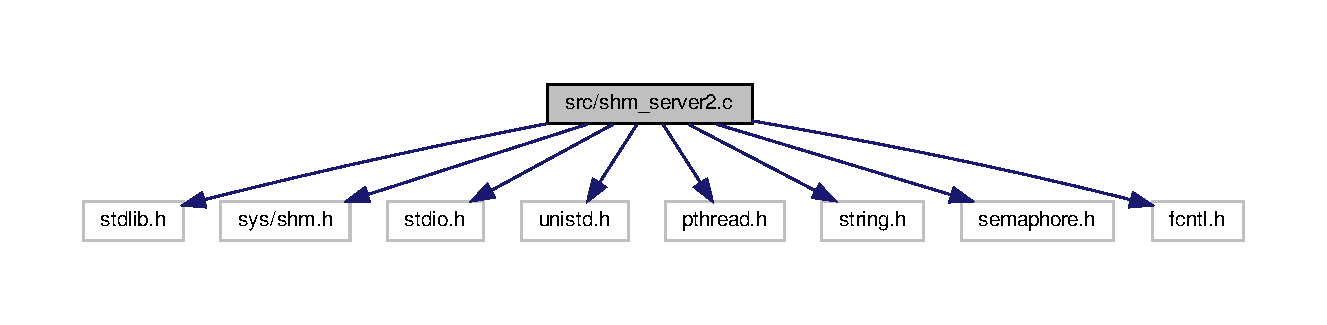
\includegraphics[width=350pt]{shm__server2_8c__incl}
\end{center}
\end{figure}
\subsection*{Classes}
\begin{DoxyCompactItemize}
\item 
struct \hyperlink{structshmseg}{shmseg}
\begin{DoxyCompactList}\small\item\em this is the message structure containing the id of the message writer and the message \end{DoxyCompactList}\end{DoxyCompactItemize}
\subsection*{Functions}
\begin{DoxyCompactItemize}
\item 
void $\ast$ \hyperlink{shm__server2_8c_af825808a184ae13bc67c961b0ed1a377}{func\+\_\+write} (void $\ast$args)
\item 
void $\ast$ \hyperlink{shm__server2_8c_ace3f9ecb971163860b43eb90bcd75ff2}{func\+\_\+read} (void $\ast$args)
\item 
int \hyperlink{shm__server2_8c_ae66f6b31b5ad750f1fe042a706a4e3d4}{main} ()
\end{DoxyCompactItemize}
\subsection*{Variables}
\begin{DoxyCompactItemize}
\item 
pthread\+\_\+mutex\+\_\+t \hyperlink{shm__server2_8c_a0abaf4b5d42c4e5d19190035fade3599}{lock}
\begin{DoxyCompactList}\small\item\em this the mutex to maintain lock between the threads \end{DoxyCompactList}\end{DoxyCompactItemize}
\textbf{ }\par
\begin{DoxyCompactItemize}
\item 
sem\+\_\+t $\ast$ \hyperlink{shm__server2_8c_a31dc0ff5363c41ad195f7e27d2d10ca9}{read\+\_\+block}
\begin{DoxyCompactList}\small\item\em these are the read and write semaphore pointers to maintain exclusivity between the server and client processes \end{DoxyCompactList}\item 
sem\+\_\+t $\ast$ \hyperlink{shm__server2_8c_a1ba04b4da8bf3354235de7186f980e7c}{write\+\_\+block}
\begin{DoxyCompactList}\small\item\em these are the read and write semaphore pointers to maintain exclusivity between the server and client processes \end{DoxyCompactList}\end{DoxyCompactItemize}



\subsection{Function Documentation}
\mbox{\Hypertarget{shm__server2_8c_ace3f9ecb971163860b43eb90bcd75ff2}\label{shm__server2_8c_ace3f9ecb971163860b43eb90bcd75ff2}} 
\index{shm\+\_\+server2.\+c@{shm\+\_\+server2.\+c}!func\+\_\+read@{func\+\_\+read}}
\index{func\+\_\+read@{func\+\_\+read}!shm\+\_\+server2.\+c@{shm\+\_\+server2.\+c}}
\subsubsection{\texorpdfstring{func\+\_\+read()}{func\_read()}}
{\footnotesize\ttfamily void$\ast$ func\+\_\+read (\begin{DoxyParamCaption}\item[{void $\ast$}]{args }\end{DoxyParamCaption})}

this function is the read function used by the read thread 
\begin{DoxyParams}{Parameters}
{\em args} & it contains the address of the shared memory shared between the server and the client \\
\hline
\end{DoxyParams}
\mbox{\Hypertarget{shm__server2_8c_af825808a184ae13bc67c961b0ed1a377}\label{shm__server2_8c_af825808a184ae13bc67c961b0ed1a377}} 
\index{shm\+\_\+server2.\+c@{shm\+\_\+server2.\+c}!func\+\_\+write@{func\+\_\+write}}
\index{func\+\_\+write@{func\+\_\+write}!shm\+\_\+server2.\+c@{shm\+\_\+server2.\+c}}
\subsubsection{\texorpdfstring{func\+\_\+write()}{func\_write()}}
{\footnotesize\ttfamily void$\ast$ func\+\_\+write (\begin{DoxyParamCaption}\item[{void $\ast$}]{args }\end{DoxyParamCaption})}

this function is the write function used by the write thread 
\begin{DoxyParams}{Parameters}
{\em args} & it contains the address of the shared memory shared between the server and the client \\
\hline
\end{DoxyParams}
\mbox{\Hypertarget{shm__server2_8c_ae66f6b31b5ad750f1fe042a706a4e3d4}\label{shm__server2_8c_ae66f6b31b5ad750f1fe042a706a4e3d4}} 
\index{shm\+\_\+server2.\+c@{shm\+\_\+server2.\+c}!main@{main}}
\index{main@{main}!shm\+\_\+server2.\+c@{shm\+\_\+server2.\+c}}
\subsubsection{\texorpdfstring{main()}{main()}}
{\footnotesize\ttfamily int main (\begin{DoxyParamCaption}{ }\end{DoxyParamCaption})}

this function is the main funtion which creates the semaphores, mutex, shared memory and the threads.

\begin{DoxyReturn}{Returns}
returns 0 as return type is int 
\end{DoxyReturn}


\subsection{Variable Documentation}
\mbox{\Hypertarget{shm__server2_8c_a0abaf4b5d42c4e5d19190035fade3599}\label{shm__server2_8c_a0abaf4b5d42c4e5d19190035fade3599}} 
\index{shm\+\_\+server2.\+c@{shm\+\_\+server2.\+c}!lock@{lock}}
\index{lock@{lock}!shm\+\_\+server2.\+c@{shm\+\_\+server2.\+c}}
\subsubsection{\texorpdfstring{lock}{lock}}
{\footnotesize\ttfamily pthread\+\_\+mutex\+\_\+t lock}



this the mutex to maintain lock between the threads 

\mbox{\Hypertarget{shm__server2_8c_a31dc0ff5363c41ad195f7e27d2d10ca9}\label{shm__server2_8c_a31dc0ff5363c41ad195f7e27d2d10ca9}} 
\index{shm\+\_\+server2.\+c@{shm\+\_\+server2.\+c}!read\+\_\+block@{read\+\_\+block}}
\index{read\+\_\+block@{read\+\_\+block}!shm\+\_\+server2.\+c@{shm\+\_\+server2.\+c}}
\subsubsection{\texorpdfstring{read\+\_\+block}{read\_block}}
{\footnotesize\ttfamily sem\+\_\+t$\ast$ read\+\_\+block}



these are the read and write semaphore pointers to maintain exclusivity between the server and client processes 

\mbox{\Hypertarget{shm__server2_8c_a1ba04b4da8bf3354235de7186f980e7c}\label{shm__server2_8c_a1ba04b4da8bf3354235de7186f980e7c}} 
\index{shm\+\_\+server2.\+c@{shm\+\_\+server2.\+c}!write\+\_\+block@{write\+\_\+block}}
\index{write\+\_\+block@{write\+\_\+block}!shm\+\_\+server2.\+c@{shm\+\_\+server2.\+c}}
\subsubsection{\texorpdfstring{write\+\_\+block}{write\_block}}
{\footnotesize\ttfamily sem\+\_\+t $\ast$ write\+\_\+block}



these are the read and write semaphore pointers to maintain exclusivity between the server and client processes 


%--- End generated contents ---

% Index
\backmatter
\newpage
\phantomsection
\clearemptydoublepage
\addcontentsline{toc}{chapter}{Index}
\printindex

\end{document}
